\documentclass[]{rptuseminar}

% Specify that the source file has UTF8 encoding
\usepackage[utf8]{inputenc}
% Set up the document font; font encoding (here T1) has to fit the used font.
\usepackage[T1]{fontenc}
\usepackage{lmodern}

% Load language spec
\usepackage[american]{babel}
% German article --> ngerman (n for »neue deutsche Rechtschreibung«)
% British English --> english

% Ffor bibliography and \cite
\usepackage{cite}

% AMS extensions for math typesetting
\usepackage[intlimits]{mathtools}
\usepackage{amssymb}
% ... there are many more ...


% Load \todo command for notes
\usepackage{todonotes}
% Sebastian's favorite command for large inline todonotes
% Caveat: does not work well with \listoftodos
\newcommand\todoin[2][]{\todo[inline, caption={2do}, #1]{
		\begin{minipage}{\linewidth-1em}\noindent\relax#2\end{minipage}}}

% Load \includegraphics command for including pictures (pdf or png highly recommended)
\usepackage{graphicx}

% Typeset source/pseudo code
\usepackage{listings}

% Load TikZ library for creating graphics
% Using the PGF/TikZ manual and/or tex.stackexchange.com is highly adviced.
\usepackage{tikz}
% Load tikz libraries needed below (see the manual for a full list)
\usetikzlibrary{automata,positioning}

% Load \url command for easier hyperlinks without special link text
\usepackage{url}

% Load support for links in pdfs
\usepackage{hyperref}

% Defines default styling for code listings
% \definecolor{pink}{rgb}{}
\definecolor{green_ulises}{rgb}{0.2,0.75,0}
\lstdefinelanguage{smtlib2} {
  morekeywords={set-logic, declare-const, assert, check-sat, get-model},
  sensitive=true,
  morecomment=[l]{;},
  morestring=[b]"
}

\lstset{%
  columns=flexible,
  keepspaces=true,
  tabsize=3,
  basicstyle={\fontfamily{tx}\ttfamily\small},
  stringstyle=\color{green_ulises},
  commentstyle=\color{black!80}
  identifierstyle=\slshape{},
  keywordstyle=\bfseries,
  numberstyle=\small\color{pink},
  backgroundcolor=\color{gray!5},
  numberblanklines=false,
  inputencoding={utf8},
  showstringspaces=false,
  belowskip=-1mm,
  escapeinside={//*}{\^^M} % Allow to set labels and the like in comments
}

% Defines a custom environment for indented shell commands
\newenvironment{displayshellcommand}{%
	\begin{quote}%
	\ttfamily%
}{%
	\end{quote}%
}

%%%%%%%%%%%%%%%%
\lstnewenvironment{haskell}{
  \vspace{1em}%
  \lstset{
    language=Haskell,
    columns=flexible,
    keepspaces=true,
    tabsize=3,
    basicstyle={\fontfamily{tx}\ttfamily\small},
    stringstyle=\color{green_ulises},
    commentstyle=\color{black!80},
    identifierstyle=\slshape{},
    keywordstyle=\bfseries,
    numberstyle=\small\color{pink},
    backgroundcolor=\color{gray!5},
    numberblanklines=false,
    inputencoding={utf8},
    belowskip=-1mm,
    escapeinside={//*}{\^^M} % Allow to set labels and the like in comments
  }
}{
  \vspace{1em}
}%%%%%%%%%%%%%%%%%%%%%%%%%%%%%%%%%%%%%%%%%%%%%%%%%%%%%%%%%%%%%%%

\title{Liquid Haskell}
\event{Seminar: Programming Languages in Winter term 2024/2025}
\author{Mehran Shahidi, Saba Safarnezhad
  \institute{Rheinland-Pfälzische Technische Universität Kaiserslautern-Landau, Department of Computer Science}}

%%%%%%%%%%%%%%%%%%%%%%%%%%%%%%%%%%%%%%%%%%%%%%%%%%%%%%%%%%%%%%%%%%%%%%%%%%%%%%%
\begin{document}
%%%%%%%%%%%%%%%%%%%%%%%%%%%%%%%%%%%%%%%%%%%%%%%%%%%%%%%%%%%%%%%%%%%%%%%%%%%%%%%

\maketitle

%%%%%%%%%%%%%%%%%%%%%%%%%%%%%%%%%%%%%%%%%%%%%%%%%%%%%%%%%%%%%%%%%%%%%%%%%%%%%%%

\begin{abstract}
  This report gives a brief overview of \textsc{LiquidHaskell}, a tool that extends Haskell with refinement types. 
  Refinement types are types that extends expressiveness of Haskell types systems by providing predicates that can verify
  invarients of the program. This report explains briefly how SMT solvers leveraged by \textsc{LiquidHaskell} and 
  how to use \textsc{LiquidHaskell} by providing some examples. Finally, we discuss the limitations of \textsc{LiquidHaskell} and compare it with other tools.
\end{abstract}

%%%%%%%%%%%%%%%%%%%%%%%%%%%%%%%%%%%%%%%%%%%%%%%%%%%%%%%%%%%%%%%%%%%%%%%%%%%%%%

\section{Introduction}
\label{sec:introduction}
Programming verfication is an important step in software developments. It is the process of
verifying that a program behaves as it expected. There has been a lot of research in this 
area and many tools have been developed. 
Type safety is one of the important features of programming languages that helps to prevent runtime errors.
Despite catching many errors at compile time, type systems are not powerful enough to catch all the errors.
On the other, testing is another way to verify the program, but it is not always possible to test all the possible inputs.
Consider the following example:

\begin{haskell}
  average    :: [Int] -> Int
  average xs = sum xs `div` length xs
\end{haskell}

The example above is a simple function that calculates the average of a list of integers. This can be a source of runtime
error if the list is empty. While this can be caught by testing, it is not always possible to test all the possible inputs.
Another way to verify the program is to use program verification tools. These tools use mathematical logic to check the program.
One of such tools that is used in Haskell programming language is \textsc{LiquidHaskell}. \textsc{LiquidHaskell} 
(LH) extends Haskell with refinement types which are types that extend the expressiveness of Haskell.
With refinement types, we can provide invariant that the program should satisfy. 

In this report, after a short backgrouund on program verfication using SMT in section \ref{sec:background}, we will explain 
how LH works and how it uses SMT solvers to 
verify the program in section \ref{sec:lh}. Then in section \ref{sec:example} we will provide some examples how to use 
LH to verify persistent stack. Finally in section \ref{sec:conclusions} we 
discuss the limiations of LH and compare it with other tools.

% E.~g.~ 
% ``quoting'' is done by using two backticks and two single quotes

\section{Background}
\label{sec:background}
\begin{description}
  \item[Refinement Types] Refinement types add predicates to the types \cite{jhala_programming_2020}. For example, consider the following type:


    \begin{haskell}
      {-@ incr :: Pos -> Pos @-}
      incr :: Int -> Int
      incr x = x + 1
    \end{haskell}

  \item[Predicate] Predicates are haskell expressions that evaluate to boolean.
  \item[SMT Solvers] SMT solvers are used to check the satisfiability of the predicates. 
  
\end{description}
\subsection{SMT Solvers}
SMT (Satisfiability Modulo Theories) solvers are tools that can check the satisfiability of logical formulas in a specific theory.
SMT solvers extends the concept of SAT solvers by adding theories (e.g., the theory of equality, 
of integer numbers, of real numbers, of arrays, of lists, and so on) to the boolean logic \cite{clarke_satisfiability_2018}.
While SAT solvers can only check the satisfiability of boolean formulas, SMT solvers can check the satisfiability of formulas 
that contain variables from different theories. 
As an example, consider the following formula:

\begin{equation}
  \varphi = (x \lor y) \land (\lnot x \lor z)
\end{equation}

SAT solver can check the satisfiability of the formula \(\varphi\) by checking if there is an assignment for the variables \(x, y, z\).
For instance, \(x = true, y = false, z = true\) is an assignment that makes \(\varphi\) \(true\). 

On the other hand, SMT solvers can check the satisfiability of formulas that contain variables that required arithmetic theory as following formula:
Figure \ref{fig:scholar}

\begin{equation}
  x + y \leq 10 \quad and \quad x = y - 7
\end{equation}

\subsection{Z3 SMT Solvers}
\subsubsection*{Overall System Architecture of Z3}
The overall system architecture of Z3 is aimed at efficiently solving Satisfiability Modulo Theories (SMT) problems. Here's a detailed breakdown of the major components and their interactions:

 \begin{figure}[ht]
  \begin{center}
    \fbox{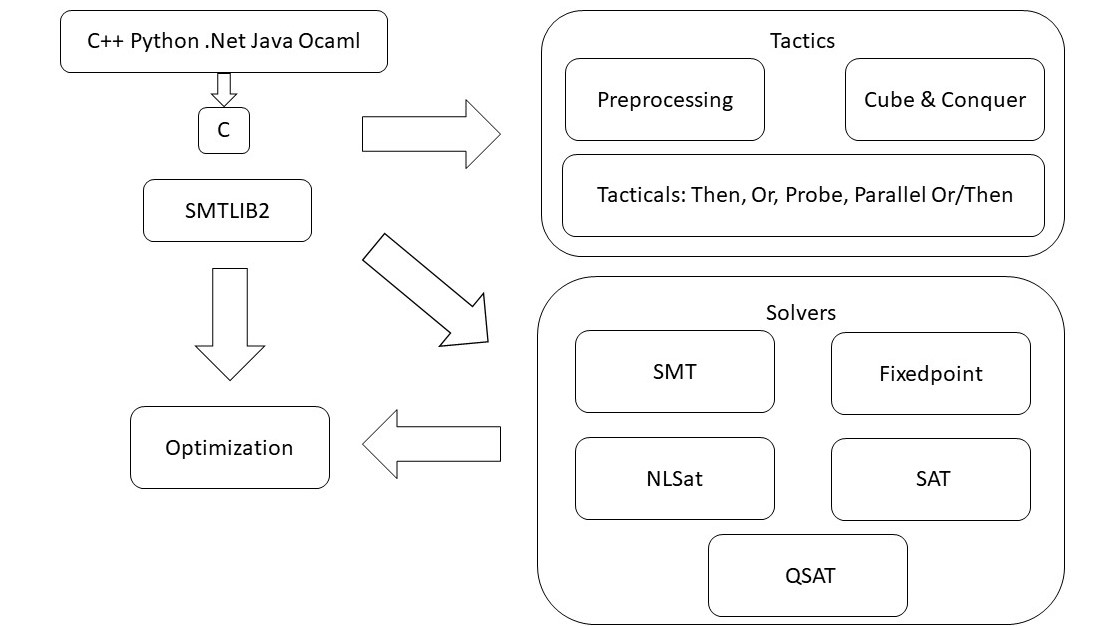
\includegraphics[width=.9\linewidth]{SMT}}%
    % fbox for "framed box"
  \end{center}
  \caption{%
     Overall system architecture of Z3
    \cite{nikolaj_bjorner_programming_nodate}
  }
  \label{fig:scholar} % NOTE: \label must appear after \caption
\end{figure}

\subsubsection{Interfaces to Z3}
Z3 can be interacted with using SMT-LIB2 scripts supplied as text files or through a pipe.
Besides this, high-level programming languages can make API calls to Z3, which are proxies
for calls over a C-based API.
\cite{nikolaj_bjorner_programming_nodate}

\subsubsection{Logical Formulas}
Z3 accepts logical formulas built from atomic variables and logical connectives, which can include symbols defined by various theories.
These formulas use basic building blocks like Boolean variables, integers, and reals, combined with logical operators such as
\texttt{And}, \texttt{Or}, \texttt{Not}, \texttt{Implies}, and \texttt{Xor}. Z3 handles complex logical expressions by
integrating symbols from multiple theories, such as arrays and arithmetic, allowing it to model a wide range of problems.
The formulas generally follow the SMT-LIB2 standard, ensuring interoperability between different SMT solvers. 
This versatility makes Z3 a powerful tool for solving diverse logical problems efficiently.
\cite{nikolaj_bjorner_programming_nodate}

\subsubsection{Theories}
Z3 supports multiple theories, including Equality and Uninterpreted Functions (EUF), Arithmetic (both linear and non-linear),
Arrays, Bit-Vectors, Algebraic Datatypes, Sequences, and Strings. Each theory has specialized decision procedures for solving
related formulas.
\cite{nikolaj_bjorner_programming_nodate}

\subsubsection{Solver}
Z3 provides services for deciding the satisfiability of formulas. This includes handling incrementality, scopes, assumptions, 
cores, models, and other methods like statistics, proofs, and retrieving solver state. Specialized solvers are included for 
different types of problems.
\cite{nikolaj_bjorner_programming_nodate}

\subsubsection*{SMT Solver}
The SMT solver in Z3 is a general-purpose solver that integrates various theories to decide the satisfiability of logical formulas. 
It uses the CDCL(T) architecture, which combines Conflict-Driven Clause Learning (CDCL) with theory solvers.
\cite{nikolaj_bjorner_programming_nodate}

\subsubsection*{Fixedpoint Solver}
The Fixedpoint solver in Z3 is used for reasoning about recursive definitions and fixed-point computations. 
It includes a Datalog engine and supports relational algebra and Property Directed Reachability (PDR) algorithms.
\cite{nikolaj_bjorner_programming_nodate} 

\subsubsection*{NLSat Solver}
The NLSat solver is specialized for non-linear arithmetic problems. 
It uses a combination of algebraic methods and SAT solving techniques to handle polynomial constraints.
\cite{nikolaj_bjorner_programming_nodate}

\subsubsection*{SAT Solver}
The SAT solver in Z3 is designed for propositional logic problems. It uses advanced techniques like in-processing 
and co-processing to efficiently solve Boolean satisfiability problems.
\cite{nikolaj_bjorner_programming_nodate}

\subsubsection*{QSAT Solver}
The QSAT solver handles quantified Boolean formulas (QBF). It extends the capabilities of the SAT solver to deal with quantifiers, 
providing solutions for more complex logical problems.
\cite{nikolaj_bjorner_programming_nodate}


\subsubsection{Tactics}
Tactics in Z3 are used for preprocessing, formula simplification, and the generation of sub-goals. they
are essential to decompose complex problems into relatively simple fragments. The preprocess tactics simplify the input formulae before they are fed into the main solver. It can include heuristics such as the propagation of constants, arithmetic simplification, and removal of redundant constraints. The Cube and Conquer tactic is used to split the search space into smaller sub-problems. (cubes) that can be solved independently. This is a very useful scheme for parallel solving
and the sum time required to solve, it greatly shortens. Tacticals are combiners which make composition of multiple tactics.
\cite{nikolaj_bjorner_programming_nodate}
\subsubsection{Optimization}
Z3 allows the use of optimization services along with user-defined problems in order to study the satisfiability of the problem while maximizing or minimizing objective functions. This applies to those problems which require solutions that are to be optimized under given constraints.
\cite{nikolaj_bjorner_programming_nodate}

\subsubsection{Applications and Example of Z3}
Software analysis verification and symbolic execution along with software analysis verification rely heavily on making use of the Z3 platform. Z3 operates through SMT-LIB2 scripts for textual logical problem inputs as well as program application interfaces using Python fundamental sources and C++ constructs and OCaml programming code. Both Z3 users prefer the Python API because of its straightforward nature and SMT-LIB2 stands out for presenting logical problems with predefined logics including arithmetic, arrays and bit-vectors.
\vspace{1em}

To be sure, consider \ref{eq:example-sat} and its satisfiability problem,
we are wondering is there a value assignment of Boolean variables Tie, Shirt,
such that three clauses conjuction :


\begin{equation}
  \label{eq:example-sat}
  (Tie \lor Shirt) \land (\lnot Tie \lor Shirt) \land (\lnot Tie \lor \lnot Shirt)
\end{equation}

Formula \ref{eq:example-sat}  can be solved in SMTLIB2 as following code:

\begin{figure}[ht]
  \begin{lstlisting} [language=SMTlIB2]
    (set-logic QF_UF)
    (declare-const Tie Bool)
    (declare-const Shirt Bool)
    (assert (or Tie Shirt))
    (assert (or (not Tie) Shirt))
    (assert (or (not Tie) (not Shirt)))
    (check-sat)
    (get-model)
  \end{lstlisting}
  \end{figure}

  When we run this, Z3 responds:
\begin{lstlisting} [language=SMTlIB2]
 sat
 (model
   (define-fun Tie () Bool false)
   (define-fun Shirt () Bool true)
 )
\end{lstlisting}
\vspace{1em}

  This SMT-LIB2 script sets up the problem, declares the variables, asserts the constraints, checks for satisfiability, and retrieves the model, just like the Python code does for Formula \ref{eq:example-sat}  with z3 in the following example.

\begin{figure}[ht]
\begin{lstlisting}[language=Python]
  from z3 import Bools, Solver, Or, Not
  Tie, Shirt = Bools('Tie Shirt')
  s = Solver()
  s.add(Or(Tie, Shirt),
        Or(Not(Tie), Shirt),
        Or(Not(Tie), Not(Shirt)))
  print(s.check())
  print(s.model())
\end{lstlisting}
\end{figure}

\vspace{1em}
The output of the code is:
\begin{lstlisting}[language=Python]
sat

[Tie = False, Shirt = True]
\end{lstlisting}
\vspace{1em}


When calling s.check(), the solver determines that the assertions are satisfiable (sat)—meaning there is a way to assign values to Tie and Shirt that makes all the conditions true. One possible solution is Tie = false and Shirt = true, which can be retrieved using s.model().
\vspace{1em}



The next example shows how Z3 reasons across multiple mathematical theories such as array theory, arithmetic, and uninterpreted functions. Z3's API analyzes the following Python snippet:


\begin{lstlisting}[language=Python]
Z = IntSort()
f = Function('f', Z, Z)
x, y, z = Ints('x y z')
A = Array('A', Z, Z)
fml = Implies(x + 2 == y, f(Store(A, x, 3)[y - 2]) == f(y - x + 1))
solve(Not(fml))

unsat
\end{lstlisting}



\paragraph{Theories Involved}
The integrated theories enabling this reasoning are:

\begin{itemize}
    \item \textbf{Linear Integer Arithmetic (LIA)}: Handles integer constraints:
    \begin{equation*}
        x + 2 = y \quad \text{and} \quad y - x + 1
    \end{equation*}
    
    \item \textbf{Array Theory}: Manages array operations through \texttt{Store} and select operators:
    \begin{equation*}
        \texttt{Store}(A, x, 3)[y - 2] \equiv \text{ite}(y - 2 = x, 3, A[y - 2])
    \end{equation*}
    where \text{ite} denotes the if-then-else operator.
    
    \item \textbf{Uninterpreted Functions}: Treats function $f$ as a black box respecting functional consistency:
    \begin{equation*}
        \forall a, b: (a = b) \implies (f(a) = f(b))
    \end{equation*}
\end{itemize}

This example illustrates Z3's theory combination mechanism, which:
\begin{itemize}
    \item Ensures coherence across different mathematical domains
    \item Handles cross-theory constraints (e.g., array indices as arithmetic expressions)
    \item Enables verification of systems with mixed abstractions (memory, arithmetic, and black-box components)
\end{itemize}

This capability makes Z3 particularly useful for software verification, as real-world programs inherently integrate these concepts \cite{nikolaj_bjorner_programming_nodate}.
\section{Working with LiquidHaskell}
\label{sec:lh}
LH is a tool that extends Haskell with refinement types. Refinement types are types that extend the expressiveness of Haskell types systems by providing predicates that can verify invarients of the program. In this section, we will explain how to use LH and how it works.
LH is available as a GHC plugin. To use LH, you need to add LH dependecy to the cabal file as following:

\vspace{1em}
\begin{lstlisting}
 cabal-version: 1.12

 name:           lh-plugin-demo
 version:        0.1.0.0
 ...
 ...
   build-depends:
       liquid-prelude,
       liquid-vector,
       liquidhaskell,
       base,
       containers,
       vector
   default-language: Haskell2010
   ghc-options:  -fplugin=LiquidHaskell
\end{lstlisting}
\vspace{1em}

By adding this dependency, LH can now check your program at compile time or via code linter in your IDE of choice. In following sections, we will explain how to use LH to verify the program.
\subsection{Type Refinement}
Refinement types allows to constrain the type of the variables by adding predicates to the types \cite{jhala_programming_2020}. For example we can define natural numbers as following:

\begin{haskell}
 {-@ type Nat = {v:Int | 0 <= v} @-}
\end{haskell}

Now if you configure your IDE to use Haskell LSP, it will show following error if you try to assign a negative number to a variable of type Nat.
\begin{haskell}
 {-@ x :: Nat @-}
 x = -1
 >>> typecheck: Liquid Type Mismatch
   .
   The inferred type
     VV : {v : GHC.Types.Int | v == GHC.Num.negate (GHC.Types.I# 1)
                               && v == (-GHC.Types.I# 1)}
   .
   is not a subtype of the required type
     VV : {VV##493 : GHC.Types.Int | VV##493 >= 0}
   .
   Constraint id 2
\end{haskell}
The error message shows that the inferred type of the variable x is not a subtype of the required type.

Using refinement types, one can define pre-conditions and post-conditions of the functions\cite{jhala_programming_2020}. 
For example, consider the following function:

\begin{haskell}
 tail :: [a] -> [a]
 tail (_:xs) = xs
 tail [] = error "tail: empty list"
\end{haskell}

The function defined above is a partial function because it does not handle the case when the list is empty. 
Typicall haskell types only allow to introduce the \textit{Maybe} type which postpone the handling of error to the other 
part of the program \cite{jhala_programming_2020}. Using refinement types, we can define the type of tail function as following:

\begin{haskell}
 {-@ tail :: {v:[a] | 0 < len v} -> a @-}
 tail :: [a] -> [a]
 tail (x:_) = x
\end{haskell}

Now our function is a total function as it doesn't allow non-empty list to be passed to \textit{tail}. However, it can't 
check the following case.

\begin{haskell}
 x :: [Int]
 x = tail (tail [1, 2])
\end{haskell}

When calling functions, LH won't look into the body of function to see if the first application of \textit{tail} gives the valid non-empty list to the second \textit{tail}.
To allow LH consider the above example as safe, we need to also specify post-condition for our function as following:

\begin{haskell}
 {-@ tail :: xs: {v:[a] | 0 < len v} -> {v:[a] | len v == len xs - 1} @-}
 tail :: [a] -> [a]
 tail (x:_) = x
\end{haskell}
\subsection{Refined Data Types}
In the above examples, we saw how refinements of input and output of fucntion allows us to have stronger arguments about our program. 
We can take this further by refining the data types. Consider the following example:

\begin{haskell}
  data Slist a = Slist { size :: Int, elems :: [a] }

  {-@ data Slist a = Slist { size :: Nat, elems :: {v:[a] | len v == size} } @-}
\end{haskell}

In the above example, we introduced a new data type \textit{Slist} which is a list with a size. 
We also added a refinement to the data type that ensures that the size of the list is equal to the length of the list. 
This ensures that the size of the list is always correct.

The only thing in above example that is missing is the definition of \textit{len}. Fortunately, this function has already reflected by
LH. In the following section, we show how can we use reflection or measure directives to define and execute any user defined haskell function in the refinement logic and
reason about them.

\subsection{Lifting Functions to the Refinement Logic}
When our programs become more complex, we need to define our own functions in the refinement logic and reason about
a function within another function. In LH, we can define our own functions in the refinement logic using reflection.
There are two ways to define a function in the refinement logic: \texttt{reflection} and \texttt{measure}. 

\texttt{Measure} can be used on a function with one argument that is pattern matched in the function body. Then, the
LH copies the function to the refinement logic, adds a refinement type to the constructor of the function's argument, and emits inferred global
invariants related to the refinement. Consider the following example:

\begin{haskell}
data Bag a = Bag { toMap :: M.Map a Int } deriving Eq
{-@ measure bag @-}
{-@ bag :: Ord a => List a -> Bag a @-}
bag :: (Ord a) => List a -> Bag a
bag Emp = B.empty
bag (Cons x xs) = B.put x (bag xs)
\end{haskell}

\begin{haskell}
 {-# OPTIONS_GHC -fplugin=LiquidHaskell #-}

 {-@ type Pos = {v:Int | 0 < v} @-}

 {-@ incr :: Pos -> Pos @-} //*\label{srcline:typerefinement}
 incr :: Int -> Int
 incr x = x + 1 
\end{haskell}

\subsection{Verification}


\section{Example Application}

In this section, we discuss the insertion sort algorithm and how to verify its functional correctness using LiquidHaskell. Insertion sort is a simple sorting algorithm that builds the final sorted list one element at a time. Using LiquidHaskell, we aim to ensure that the sorted list is both ordered and a permutation of the input.

\subsection{Definition of Insertion Sort}

Insertion sort is implemented in Haskell with two main components: the \texttt{insert} function, which places an element in its correct position in a sorted list, and the \texttt{insertSort} function, which recursively sorts the input list. Below is the Haskell implementation:

\begin{lstlisting}[caption=Insertion Sort Implementation]
{-@ LIQUID "--reflection" @-}
{-@ LIQUID "--ple" @-}

module InsertionSort where

-- Define the List type
data List a = Emp | Cons a (List a) deriving (Eq, Show)

-- Insert operation
{-@ reflect insert @-}
insert :: (Ord a) => a -> List a -> List a
insert x Emp = Cons x Emp
insert x (Cons y ys)
  | x <= y    = Cons x (Cons y ys)
  | otherwise = Cons y (insert x ys)

-- Insertion Sort operation
{-@ reflect insertSort @-}
insertSort :: (Ord a) => List a -> List a
insertSort Emp = Emp
insertSort (Cons x xs) = insert x (insertSort xs)
\end{lstlisting}

\subsection{Specification}

To verify the correctness of the insertion sort, we define specifications that ensure the following:
1. The output list is sorted.
2. The output list is a permutation of the input list.

\subsubsection{Sortedness Specification}

We define a helper function, \texttt{isSorted}, to check whether a list is sorted:

\begin{lstlisting}[caption=Sortedness Helper Function]
{-@ reflect isSorted @-}
isSorted :: (Ord a) => List a -> Bool
isSorted Emp = True
isSorted (Cons x xs) =
  isSorted xs && case xs of
    Emp        -> True
    Cons x1 _  -> x <= x1
\end{lstlisting}

The \texttt{isSorted} function is then used to specify and verify the correctness of the \texttt{insert} and \texttt{insertSort} functions.

\subsubsection{Insert Function Specification}

The \texttt{insert} function places an element into a sorted list while maintaining its sortedness:

\begin{lstlisting}[caption=Insert Specification]
{-@ insert :: x:_ -> {xs:_ | isSorted xs} -> {ys:_ | isSorted ys} @-}
\end{lstlisting}

\subsubsection{Insertion Sort Specification}

The \texttt{insertSort} function ensures that the output is sorted and is a permutation of the input:

\begin{lstlisting}[caption=Insertion Sort Specification]
{-@ insertSort :: xs:_ -> {ys:_ | isSorted ys && bag xs == bag ys} @-}
\end{lstlisting}

Here, \texttt{bag} represents a multiset of elements, used to verify that the output is a permutation of the input.

\subsection{Proofs}

We outline proof strategies for the correctness of the \texttt{insert} and \texttt{insertSort} functions using LiquidHaskell.

\subsubsection{Proof of Insert Correctness}

The correctness of \texttt{insert} follows from its definition. We additionally define a lemma to assist in the proof:

\begin{lstlisting}[caption=Insert Lemma]
{-@ lem_ins :: y:_ -> {x:_ | y < x} -> {ys:_ | isSorted (Cons y ys)} 
    -> {isSorted (Cons y (insert x ys))} @-}
lem_ins :: (Ord a) => a -> a -> List a -> Bool
lem_ins y x Emp = True
lem_ins y x (Cons y1 ys) = if y1 < x then lem_ins y1 x ys else True
\end{lstlisting}

\subsubsection{Proof of Insertion Sort Correctness}

The correctness of \texttt{insertSort} is established by combining the correctness of \texttt{insert} and ensuring that the output satisfies both the sortedness and permutation properties.

\begin{lstlisting}[caption=Insertion Sort Proof]
{-@ insertSort :: xs:_ -> {ys:_ | isSorted ys && bag xs == bag ys} @-}
insertSort :: (Ord a) => List a -> List a
insertSort Emp = Emp
insertSort (Cons x xs) = insert x (insertSort xs)
\end{lstlisting}

By verifying these properties using LiquidHaskell, we ensure that the implementation of insertion sort is functionally correct and adheres to the desired specifications.

\section{Conclusion}
This paper demonstrates the use of LiquidHaskell to verify the functional correctness of a persistent stack. Future work includes extending this methodology to more complex data structures such as queues and deques.
\label{sec:example}

\section{Conclusions, Results, Discussion}
\label{sec:conclusions}

%%%%%%%%%%%%%%%%%%%%%%%%%%%%%%%%%%%%%%%%%%%%%%%%%%%%%%%%%%%%%%%%%%%%%%%%%%%%%%%
\newpage
\nocite{*}
\bibliographystyle{eptcs}
\bibliography{references}

%%%%%%%%%%%%%%%%%%%%%%%%%%%%%%%%%%%%%%%%%%%%%%%%%%%%%%%%%%%%%%%%%%%%%%%%%%%%%%%
\end{document}
%%%%%%%%%%%%%%%%%%%%%%%%%%%%%%%%%%%%%%%%%%%%%%%%%%%%%%%%%%%%%%%%%%%%%%%%%%%%%%%
